\documentclass{beamer}
\usepackage{algorithm}
\usepackage[noend]{algpseudocode}
\usepackage{listings}
\usepackage{courier}
\lstset{
  language=,
  basicstyle=\footnotesize\ttfamily,
  numberstyle=\tiny,
  numbersep=5pt,
  tabsize=2,
  extendedchars=true,
  breaklines=true,
  %frame=b,
  keywordstyle=\color{red},
  stringstyle=\color{blue}\ttfamily,
  %t@github.com:psanan/gittutorial-demo.gitcommentstyle=\color{greenmod},
  numberstyle=\color{violet},
  identifierstyle=\color{orange},
  showspaces=false,
  showtabs=false,
  xleftmargin=17pt,
  framexleftmargin=17pt,
  framexrightmargin=5pt,
  framexbottommargin=4pt,
  showstringspaces=false
}
\usepackage{xcolor}
\usepackage{color}
\usepackage{amsmath}

\definecolor{greenmod}{rgb}{0,0.6,0}

\hypersetup{linkcolor=magenta,colorlinks=true}

\usetheme{Madrid}
\setbeamertemplate{navigation symbols}{} % Remove the navigation symbols
\setbeamertemplate{sections/subsections in toc}[default] %Turn off ugly toc numbering
\setbeamertemplate{itemize subitem}[triangle]
\setbeamertemplate{itemize item}[triangle]
\setbeamertemplate{enumerate items}[default]
%\setbeamercovered{transparent}
\usepackage{appendixnumberbeamer}
\defbeamertemplate{section page}{customsection}[1][]{%
  \begin{centering}
    {\usebeamerfont{section name}\usebeamercolor[fg]{section name}#1}
    \vskip1em\par
    \begin{beamercolorbox}[sep=12pt,center]{part title}
      \usebeamerfont{section title}\insertsection\par
    \end{beamercolorbox}
  \end{centering}
}
\defbeamertemplate{subsection page}{customsubsection}[1][]{%
  \begin{centering}
    {\usebeamerfont{subsection name}\usebeamercolor[fg]{subsection name}#1}
    \vskip1em\par
    \begin{beamercolorbox}[sep=8pt,center,#1]{part title}
      \usebeamerfont{subsection title}\insertsubsection\par
    \end{beamercolorbox}
  \end{centering}
}
\AtBeginSection{\frame{\sectionpage}}
\AtBeginSubsection{\frame{\subsectionpage}}

%%%%%%%%%%%%%%%%%%%%%%%%%%%%%%%%%%%%%%%%%%%%%%%%%%%%%%%%%%%%%%%%%%%%%%%%%%%%%%%

\graphicspath{images/}

% clashes with beamer
%\usepackage[colorlinks=true]{hyperref}

\usepackage{booktabs}

%%%%%%%%%%%%%%%%%%%%%%%%%%%%%%%%%%%%%%%%%%%%%%%%%%%%%%%%%%%%%%%%%%%%%%%%%%%%%%%

%%%%%%%%%%%%%%%%%%%%%%%%%%%%%%%%%%%%%%%%%%%%%%%%%%%%%%%%%%%%%%%%%%%%%%%%%%%%%%%

\author{Patrick Sanan}
\institute[USI/ETHZ] 
{
USI Lugano ICS / ETH Z\"{u}rich D-ERDW\\
}

%%%%%%%%%%%%%%%%%%%%%%%%%%%%%%%%%%%%%%%%%%%%%%%%%%%%%%%%%%%%%%%%%%%%%%%%%%%%%%%

\title{A Git Tutorial} 
\subtitle[]{What it is, how you use it, and what it's good for}
\date[]{} 
% Long date messes up footer

%%%%%%%%%%%%%%%%%%%%%%%%%%%%%%%%%%%%%%%%%%%%%%%%%%%%%%%%%%%%%%%%%%%%%%%%%%%%%%%

\begin{document}

%%%%%%%%%%%%%%%%%%%%%%%%%%%%%%%%%%%%%%%%%%%%%%%%%%%%%%%%%%%%%%%%%%%%%%%%%%%%%%%%
%%%%%%%%%%%%%%%%%%%%%%%%%%%%%%%%%%%%%%%%%%%%%%%%%%%%%%%%%%%%%%%%%%%%%%%%%%%%%%%%

\begin{frame}[fragile]
\titlepage 
\begin{center}
\href{https://bitbucket.org/psanan/gittutorial}{https://bitbucket.org/psanan/gittutorial}
\end{center}
\end{frame}

%%%%%%%%%%%%%%%%%%%%%%%%%%%%%%%%%%%%%%%%%%%%%%%%%%%%%%%%%%%%%%%%%%%%%%%%%%%%%%%

\begin{frame}
\tableofcontents 
\end{frame}

\section{Who is this for?}
\begin{frame}[fragile]
\frametitle{Assumed Audience}
Assumptions about the audience:
\begin{itemize}
\item You use code
\item You sometimes feel like you're wasting your time when you work with code, especially when it comes time to collaborate
\item You know how to use a terminal, shell, terminal-based text editor, and login file on your computer \footnote{If not, ask me afterwards}
\end{itemize}
\uncover<2>{ 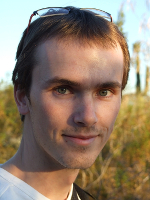
\includegraphics[width=50px]{antoine.jpg} (or you are Antoine)}
\end{frame}

\begin{frame}[fragile]
\frametitle{Purpose of this Presentation}
\begin{itemize}
\item Give an idea of the fairly simple (beautiful) data structure which git manipulates
\item Give an introduction to the (less beautiful) way you can interact with this from the command line
\item Show some of the benefits of using services like Bitbucket or GitHub
\item Give a few very simple demonstrations
\item Hopefully, convince you that these tools are worth investing the time to learn more thoroughly
\end{itemize}
\end{frame}

\section{What is git?}
\begin{frame}[fragile]
\frametitle{What is Version Control?}
\begin{itemize}
\item
git is a \emph{Version Control System (VCS)}
\item It's a system to help you keep track of the history and versions of a ``project'' (usually based on source code)
\item 
We will show how one might invent such a thing.\footnote{based on \href{http://tom.preston-werner.com/2009/05/19/the-git-parable.html}{``The Git Parable'' by Tom Preston-Werner}}
\end{itemize}
\end{frame}

\begin{frame}[fragile]
\frametitle{Tracking History - Snapshots}
\begin{itemize}
\item When working on code, it's natural to want to save certain states.
\item You might do this manually, creating folders with different \emph{snapshots} of your data every once in a while.
\end{itemize}
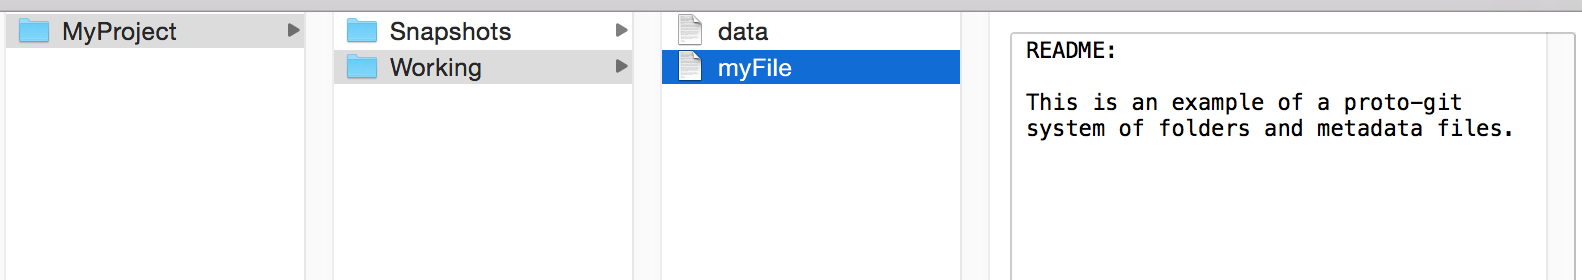
\includegraphics[scale=0.4]{snapshot1.png}\\
\vspace{10px}

\includegraphics[scale=0.4]{snapshot2.png}

\end{frame}

\begin{frame}[fragile]
\frametitle{Adding Metadata - Commits}
\begin{itemize}
\item I might decide that I want more information about each snapshot
\item I introduce data in a new folder of \emph{commits} 
\item I want to be able to ``rewind'', so I record a \emph{parent} commit for each commit (except the first)
\end{itemize}
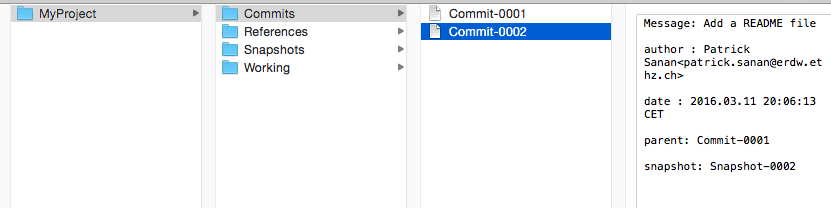
\includegraphics[scale=0.4]{commit1.png}\\
\end{frame}

\begin{frame}[fragile]
\frametitle{Adding Metadata - Commits}
\begin{itemize}
\item I also introduce a new file called \texttt{HEAD} which points to the latest commit
\item To save my state,
\begin{enumerate}
\item Copy the state indicated by \texttt{HEAD} to a \emph{staging area} and pick some or all of the changes from my \emph{working directory} to add there
\item Copy the staging area directory to a new snapshot
\item Create a new commit, using \texttt{HEAD} as the parent and pointing to my new snapshot
\item Update \texttt{HEAD} to the new commit
\end{enumerate}
\end{itemize}
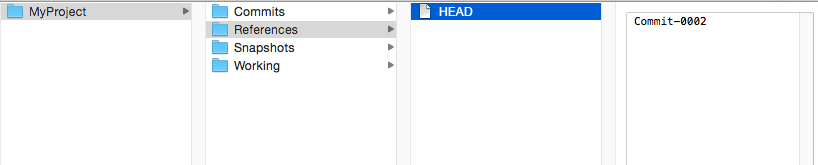
\includegraphics[scale=0.4]{commit2.png}
\end{frame}

\begin{frame}[fragile]
\frametitle{Different Versions}
\begin{itemize}
\item We can keep track of multiple versions of our project by adding more \emph{references} and updating them. 
\item We change \texttt{HEAD} to now point to one of these \emph{branches}
\item As I add new commits, I update the branch pointed to by \texttt{HEAD} to point to the new commit
\end{itemize}
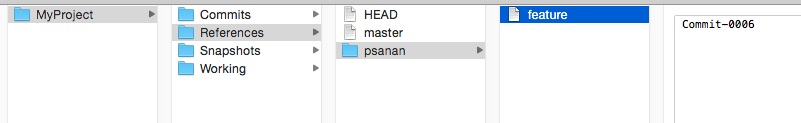
\includegraphics[scale=0.4]{branch1.png}\\
\vspace{10px}
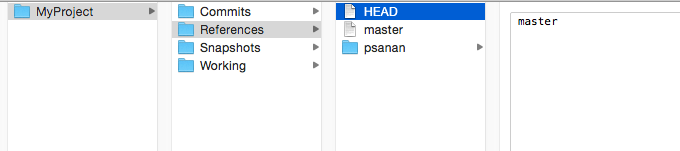
\includegraphics[scale=0.4]{branch2.png}
\end{frame}

\begin{frame}[fragile]
\frametitle{Different Versions}
\begin{itemize}
\item We realize that we can have multiple parents in a commit, which allows us to \emph{merge} branches.
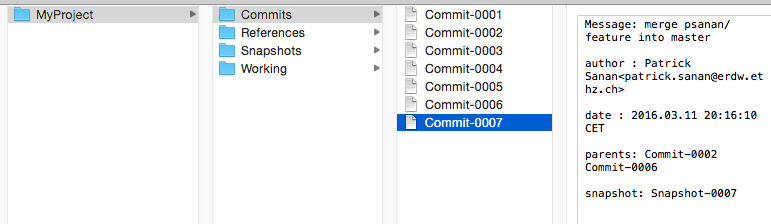
\includegraphics[scale=0.4]{branch3.png}
\end{itemize}
\end{frame}

\begin{frame}[fragile]
\frametitle{Other People}
\begin{itemize}
\item Now, suppose you and I both have a copy of this \emph{repository} (\texttt{MyProject}) and we want to collaborate.
\item We have the clever idea that we can name the files by applying a function\footnote{a \emph{cryptographic hash function}} to their contents. Now, if we have files with the same names, we have the same data.
\end{itemize}
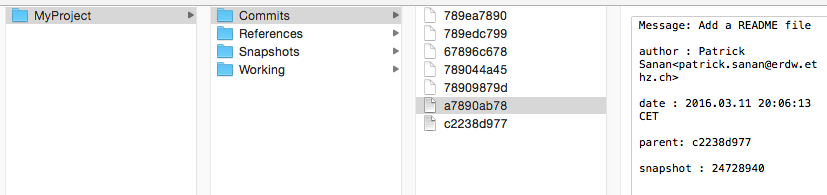
\includegraphics[scale=0.4]{remote1.png}\\
\vspace{10px}
\end{frame}

\begin{frame}[fragile]
\frametitle{Other People}
\begin{itemize}
\item I keep a special set of \emph{remote references} to branches which correspond to your repository
\item When I want your changes from a branch
\begin{itemize}
\item You send me the reference to your version of the branch.
\item I look at the reference and ask for any files (commits and snapshots) that I am missing.
\item I can make a merge commit as before. 
\item I can then send you my reference and you can repeat the steps so that we are synchronized.
\end{itemize}
\end{itemize}

\includegraphics[scale=0.3]{remote2.png}
\vspace{10px}
\end{frame}

\begin{frame}[fragile]
\frametitle{That's it!}
Git is simply software that, at its core, does all the things we just mentioned, properly implemented:
\begin{itemize}
\item Defines data in a \emph{repository}
\item Records \emph{snapshots} of a set of files
\item Gives you a way to obtain a copy of the files, edit them, and add your changes as a new snapshot.
\item Keeps track of \emph{commits} for each snapshot: a summary, who made the changes, when, and from what previous snapshot.
\item Keeps track \emph{branches}, which are pointers to commits. It provides a way to increment them, as new commits are added, and a way to merge them.
\item Keeps track of references to \emph{remote repositories} and provides a way to send and recieve repository data.
\end{itemize}
\end{frame}

\begin{frame}[fragile]
\frametitle{Aside: Differences from other Version Control Systems}
Some of you may be scarred by previous version control systems.
\begin{itemize}
\item It's very easy to set up a repository and share it with git.
\item Git (and Mercurial/Hg) are \emph{Distributed Version Control Systems}. 
\begin{itemize}
\item There is no need to be in constant contact with a central server
\item You have a copy of everything on your machine
\item Branching is cheap (just pointers)
\end{itemize}
\item It's hard to lose data with git. 
\begin{itemize}
\item
You have a complete copy of the history locally. 
\item The files in the \texttt{.git} folder are all named with cryptographic hashes, so if they are corrupted, you will find out.
\item ``Get out what you put in''.
\end{itemize}
\end{itemize}
\end{frame}

\begin{frame}[fragile]
\frametitle{A Git Repository in Graphical Form}
\begin{itemize}
\item Git repositories are commonly drawn as Directed Acyclic Graphs (DAGs) (or, imprecisely, ``trees'')
\item A commit is a node and edges from its parent(s). 
\item A branch is a box which labels a commit
\item \texttt{HEAD} is a label for a branch
\item Merges are commits with exactly two parents
\item Bitbucket, Github, and GUI tools can draw these nicely for you
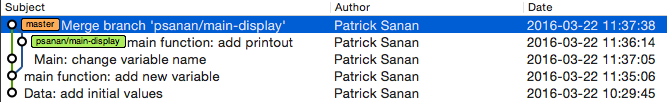
\includegraphics[width=250px]{gitx.png}\\
(Here, \texttt{HEAD} is marked by coloring the \texttt{master} branch)
\end{itemize}
Let's draw one on the board, and see what happens when we add new commits, including one which merges two branches.
\end{frame}

\section{How do I use it?}

\subsection{Basic Usage}
\begin{frame}[fragile]
\frametitle{Obtaining Git}
There are many ways to obtain git. 
\begin{itemize}
\item You can download a binary from \texttt{git-scm.com}
\item If you are using Linux, you likely already have it (if not, try \lstinline{sudo apt-get install git}).
\item You can install git from Macports or Homebrew on OS X.
\begin{lstlisting}[language=C++]
sudo port install git
brew install git
\end{lstlisting}

\end{itemize}
\end{frame}

\begin{frame}[fragile]
\frametitle{Setting Git Up}
\begin{itemize}
\item
To be able to keep track of who made which changes, git needs to know who you are.
\item 
A way to do this is to tell git these things each time you log into a terminal, by calling the \lstinline{git config} command. For instance, add commands to your \lstinline{~/.bashrc} file.
\item 
In addition to specifying your name and email address, I recommend you turn on colors and set your favorite text editor to edit commit messages.
\begin{lstlisting}[language=]
git config --global user.name "Patrick Sanan"
git config --global user.email "patrick.sanan@erdw.ethz.ch"
git config --global color.status auto
git config --global color.branch auto 
git config --global core.editor vim
\end{lstlisting}
\end{itemize}
\end{frame}

\begin{frame}[fragile]
\frametitle{Creating a Repository}
\begin{itemize}
\item From now, we'll start working on a real example. 
\item I assume that I have a working \lstinline{git} executable and that I have set up my login file to establish my identity.
\item I create a new directory and create a new git repository there:
\begin{lstlisting}[language=C++]
mkdir myDemoProject
cd myDemoProject
git init
\end{lstlisting}
\item Data is created in the \lstinline{.git} directory. Never change anything in this directory.
\item (I'll be doing everything from the terminal here, but you can also use \href{https://git-scm.com/downloads/guis}{various GUI tools} to work with git)
\end{itemize}
\end{frame}

\begin{frame}[fragile]
\frametitle{Adding and Tracking Changes to Files}
\begin{itemize}
\item \lstinline{git add} adds files to the staging area.
\item \lstinline{git commit} creates a new snapshot from staging area, creates a new commit, and updates the branch reference.
\item \lstinline{git status} lets you know the current state.
\item Try the following (use your favorite editor instead of vim)
\begin{lstlisting}[language=C++]
vim data.txt
git status
git add data.txt
git status
git commit
git log
\end{lstlisting}
\item (If you only want a short commit message, you can use \lstinline{git commit -m"Component: summary"})
\end{itemize}
\end{frame}

\begin{frame}[fragile]
\frametitle{Writing Good Commit Messages}
\begin{verbatim}
Component: summary

After a blank line, describe what you did. 
This will be something read later on by you,
and by other people trying to figure out what
broke their code. If you did something that could 
cause problems for someone, note it here. It's
also a good idea to wrap the lines yourself.
\end{verbatim}
\end{frame}

\begin{frame}[fragile]
\frametitle{What's in a commit?}
\begin{itemize}
\item For basic usage, anything you changed since the last time your code worked.
\item For work in teams or on larger projects,
\begin{itemize}
\item Changes related to a particular task on a particular component
\item Something that is reasonably atomic (can't obviously be broken down)
\item Something which won't interfere with other people's work without cause
\end{itemize}
\end{itemize}
\end{frame}

\begin{frame}[fragile]
\frametitle{Branching}
\begin{itemize}
\item By default you are on a branch called \texttt{master}
\item Create branches with \lstinline{git branch new-branch-name}
\item A good way to name branches is \lstinline{yourname/component-description}.
\item \emph{checkout} a branch with \lstinline{git checkout}. This means update \texttt{HEAD} to point to the branch, and update the working directory to the snapshot indicated by the branch.
\item Try:
\begin{lstlisting}[language=C++]
git branch psanan/data-reorganize
git checkout psanan/data-reorganize
vim data.txt
git add data.txt
git commit
git log
git checkout master
vim data.txt
git log
\end{lstlisting}
\item Common mistake: committing onto the wrong branch. Check with \lstinline{git branch} (or better yet use the git prompt mentioned later)
\end{itemize}
\end{frame}

\begin{frame}[fragile]
\frametitle{Merging and Resolving Merge Conflicts}
\begin{itemize}
\item To merge another branch into your current branch (\texttt{HEAD}), use \lstinline{git merge <branch-to-merge>}
\item Recall that a merge commit is like a normal commit, but with two parents.
\item When you merge two branches and git cannot figure out how to merge the changes, you will have to do some work. This can be frustrating.
\item Files will be specially flagged and annotated with special markers:
\begin{verbatim}
<<<<<<< HEAD
numIterations = 3;
=======
numIterations = 4;
>>>>>>> psanan/data-reorganize
\end{verbatim}
\item You must remove the special annotations and stage the file
\item Once all flagged files are staged, commit as usual
\end{itemize}
\end{frame}

\begin{frame}[fragile]
\frametitle{Resolving Merge Conflicts}
Let's perform an example with our simple repository.
\begin{lstlisting}[language=C++]
git checkout master
git merge psanan/data-reorganize
git status
vim data.txt
git add data.txt
git status
git commit
git log
\end{lstlisting}
\end{frame}

\begin{frame}[fragile]
\frametitle{States of Files}
It's worth reiterating the different states that files in your working directory can be in.
\begin{itemize}
\item They can be unmodified from the current snapshot (determined by \texttt{HEAD})
\item They can have unstaged changes
\item They can have staged changes (it is possible to stage parts of files)
\item They can be untracked
\item (They can be also be ignored if you create a special \texttt{.gitignore} file)
\item \lstinline{git status} will tell you about the states of files
\end{itemize}
\end{frame}

\begin{frame}[fragile]
\frametitle{The Most Important Commands}
We have seen most of the most important commands
\begin{itemize}
\item \lstinline{git add}
\item \lstinline{git commit}
\item \lstinline{git branch}
\item \lstinline{git checkout}
\item \lstinline{git merge}
\end{itemize}

Some more handy ones
\begin{itemize}
\item \lstinline{git help [command]}
\item \lstinline{git diff [filename]} (what's changed?)
\item \lstinline{git log -10} (see last 10 commits)
\end{itemize}
\end{frame}

\begin{frame}[fragile]
\frametitle{For (Much) More}
The Git Book : free at \href{https://git-scm.com/book}{git-scm.com/book} \\

\includegraphics[width=100px]{progit2}
\end{frame}

\subsection{Remote Repositories and Tools}

\begin{frame}[fragile]
\frametitle{Getting a Copy of an Existing Project}
\begin{itemize}
\item
The most common way to start working on a git project 
\item Make a copy of a project on GitHub or bitbucket (or somewhere else) with \lstinline{git clone}
\item You only need to know the address of the repository. You can copy it from a GitHub or bitbucket page.
\begin{lstlisting}[language=C++]
git clone git@bitbucket.org:psanan/gittutorial.git
\end{lstlisting}
\item You may have to enter your username and password
\item This creates a new local repository as a copy of the remote repository.
\item To simply obtain code with git, this is all you need to know!
\end{itemize}
\end{frame}

\begin{frame}[fragile]
\frametitle{Remote Basics (1/2)}
\begin{itemize}
\item
You can define remote repositories (\emph{remotes}) with \lstinline{git remote add <name> <address>}.
\item There are two types of addresses you can use, HTTPS and SSH. The latter will let you use an SSH key for password-free usage.
\item When you use \lstinline{git clone}, a remote is automatically created for you with the name \texttt{origin}.
\item You can have references to copies of branches on remote repositories
\item you can tell your local branches to \emph{track} remote branches. The remote branch is referred to as the \emph{upstream} branch.
\item This is set up for you for the \lstinline{master} branch when you use \lstinline{git clone} to obtain a remote repository.
\end{itemize}
\end{frame}

\begin{frame}[fragile]
\frametitle{Remote Basics (2/2)}
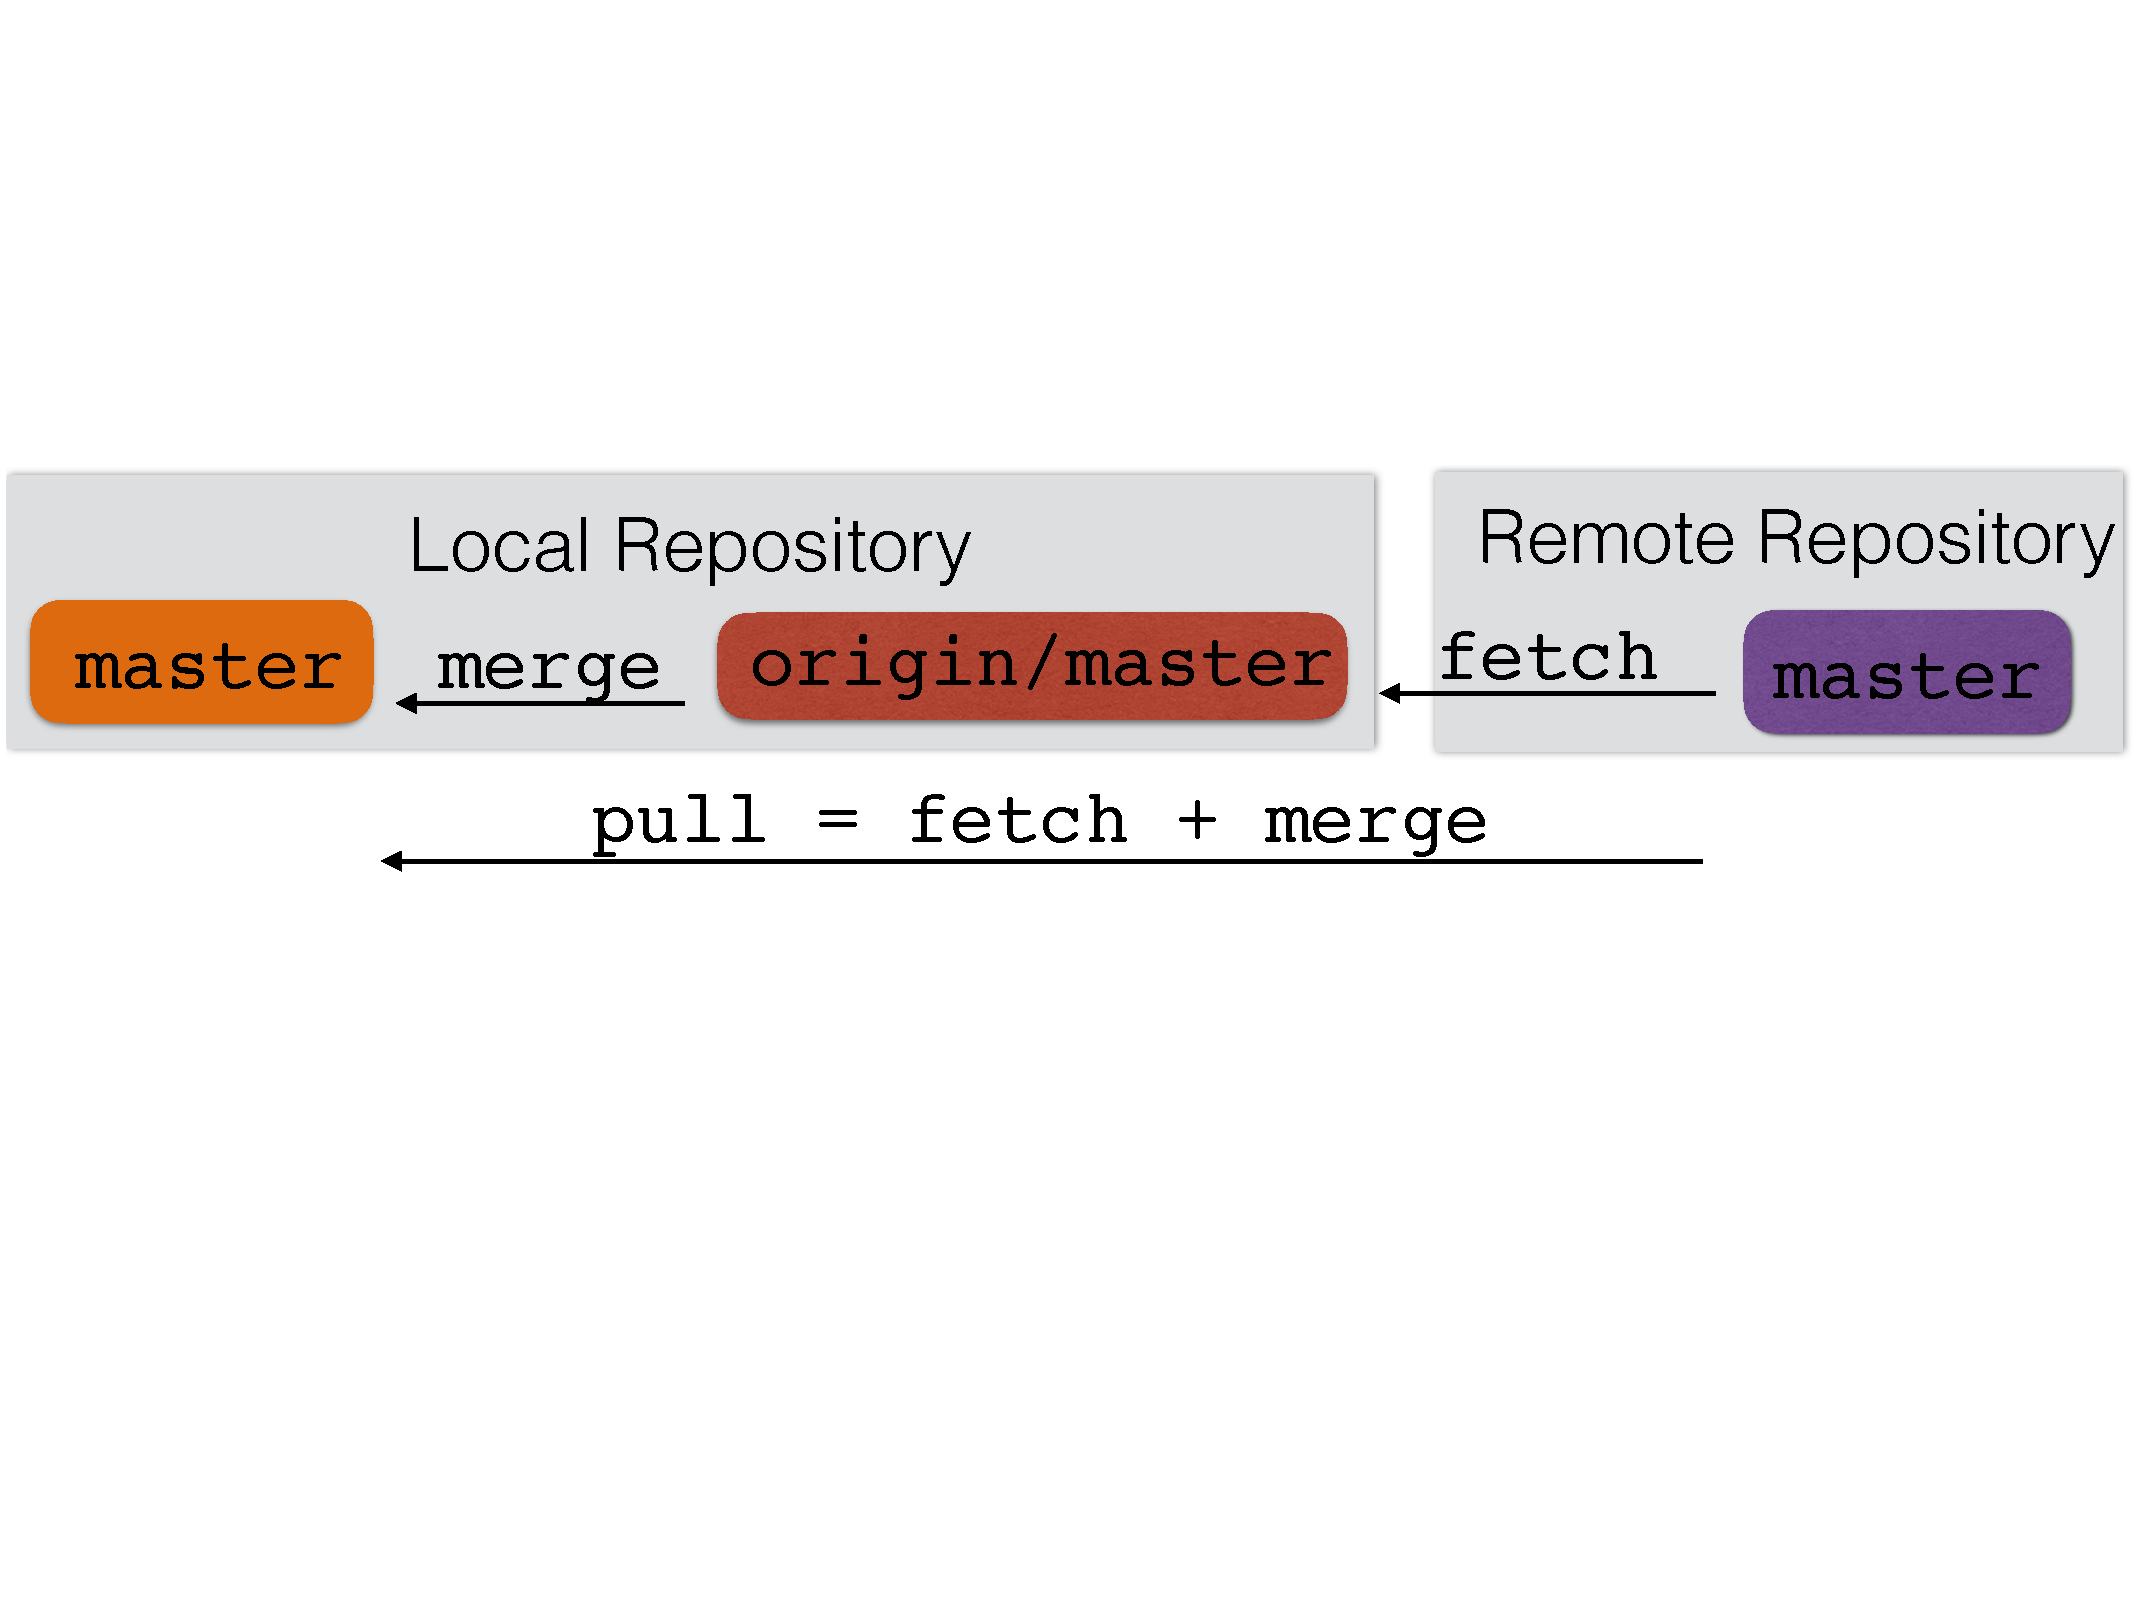
\includegraphics[width=\textwidth]{fetchcartoon}
\begin{itemize}
\item \lstinline{git fetch} updates all references from the upstream repository for the current branch.
\item \lstinline{git pull} calls \lstinline{git fetch} and also merges the remote branch into yours.
\item \lstinline{git push} sends your local branch to be merged with the remote branch.
\item \lstinline{git push -u <remotename> <branchname>} is a shortcut to push a new branch to the remote and track it.
\end{itemize}
\end{frame}

\begin{frame}[fragile]
\frametitle{An Extremely Common Mistake}
You keep local copies of remote branches in your local repository. For instance, with \lstinline{git branch -a} you might see some branches like this
\begin{lstlisting}[language=C++]
$ git branch -a
 * master
   remotes/origin/HEAD -> origin/master
   remotes/origin/master
\end{lstlisting}
When you check out a branch that is tracking a remote branch, you will see something like this:
\begin{lstlisting}[language=C++]
$ git checkout master
Switched to branch 'master'
Your branch is up-to-date with 'origin/master'.
\end{lstlisting}
This does \textbf{NOT} mean that your branch is up to date with the branch on the remote repository! It means that your branch is up to date with the \textbf{local} copy of that branch, named \lstinline{origin/master} here.
If you want to make sure you are really up to date, you must call \lstinline{git fetch} to update your local references.
\end{frame}

\begin{frame}[fragile]
\frametitle{Bitbucket and GitHub}
\begin{itemize}
\item These (freemium) services host remote git repositories for you. 
\item For both open and closed source code.
\item These repositories are essentially the same as your local ones.
\item Nice graphical overviews of your project and interactive web tools.
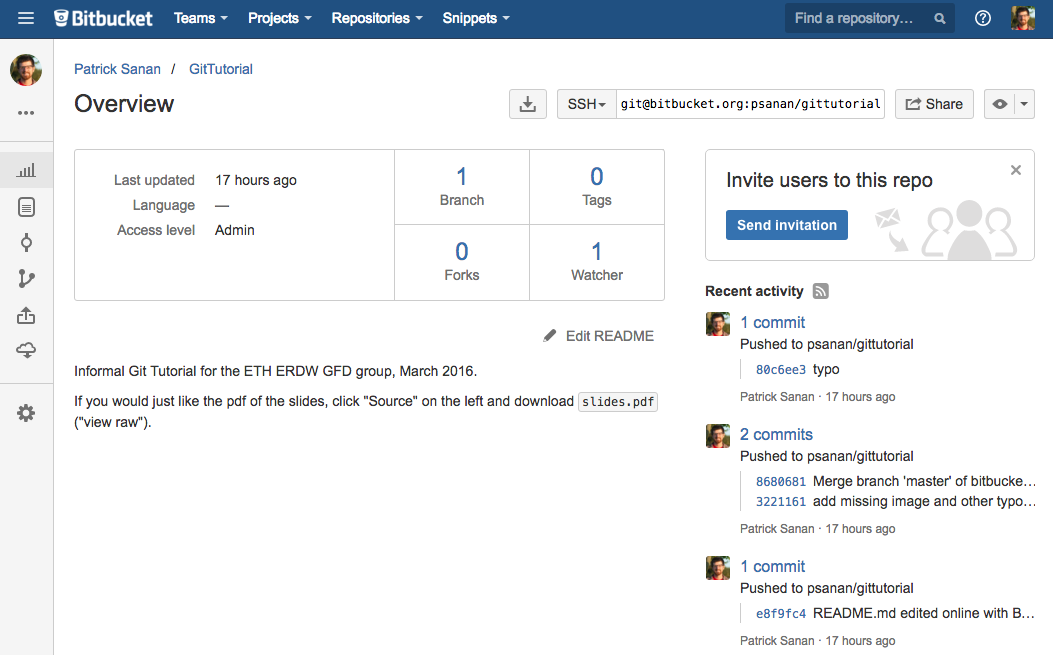
\includegraphics[scale=0.15]{bitbucket2}
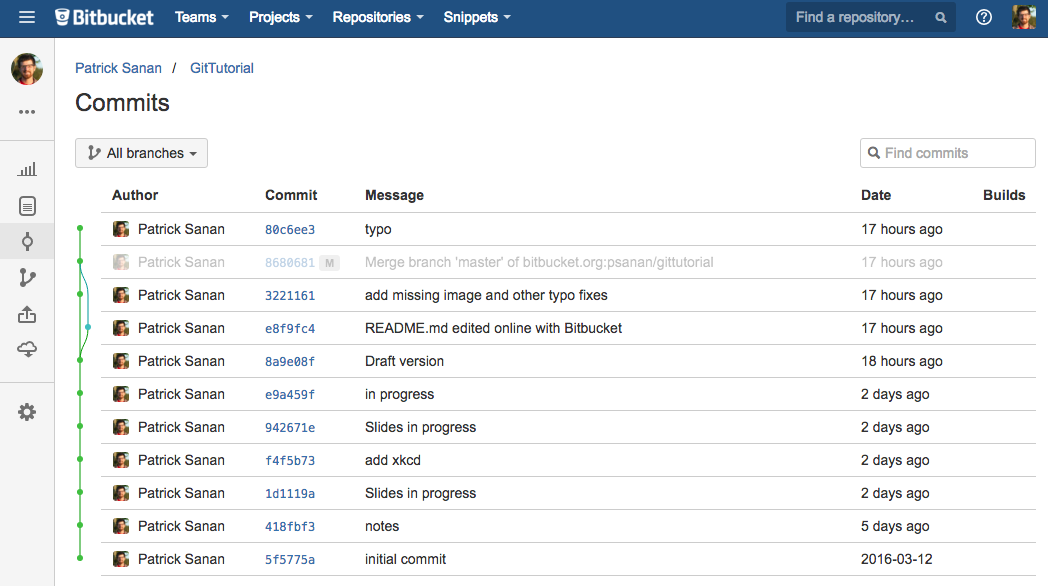
\includegraphics[scale=0.15]{bitbucket3}
\item Lots of documentation, very stable, many many users.
\end{itemize}
\end{frame}

\begin{frame}[fragile]
\frametitle{Bitbucket and GitHub}
\begin{itemize}
\item Comment directly on commits and code lines (easy code review)
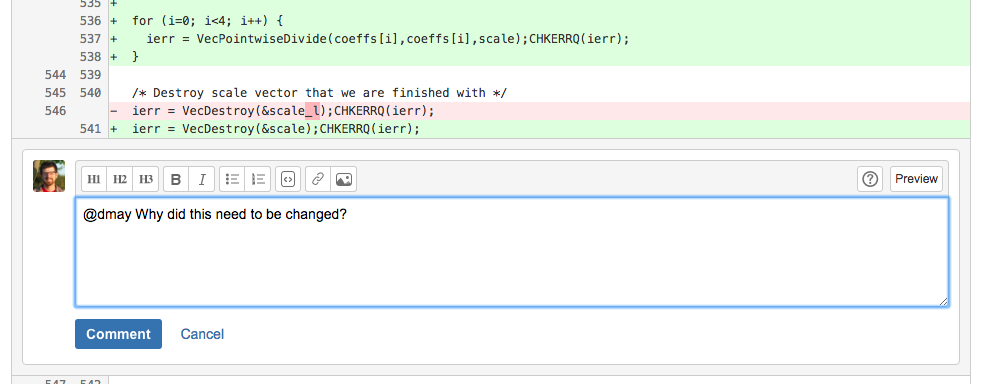
\includegraphics[scale=0.3]{bitbucket1}
\end{itemize}
\end{frame}

\begin{frame}[fragile]
\frametitle{Bitbucket and GitHub}
\begin{itemize}
\item You can receive and respond to these messages in your email program.\\
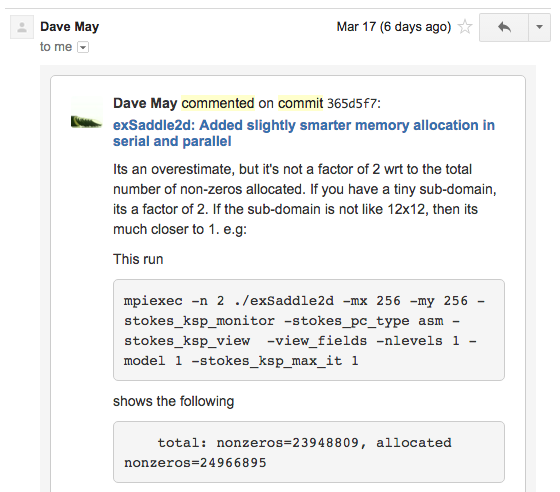
\includegraphics[scale=0.3]{bitbucket5}
\end{itemize}
\end{frame}

\begin{frame}[fragile]
\frametitle{Bitbucket and GitHub}
\begin{itemize}
\item Sign up for email notification when commits are pushed, fantastic for remote collaborations. 
\item This is currently easier on Bitbucket than GitHub.\\
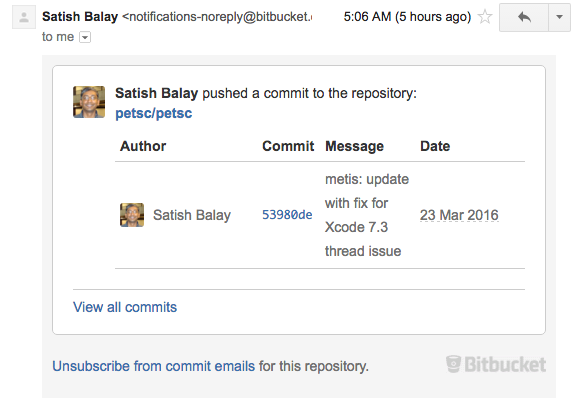
\includegraphics[scale=0.3]{bitbucket4}
\end{itemize}
\end{frame}


\begin{frame}[fragile]
\frametitle{Bitbucket and GitHub}
\begin{itemize}
\item Easily share your code, get it from anywhere, make it public when you want to. \\
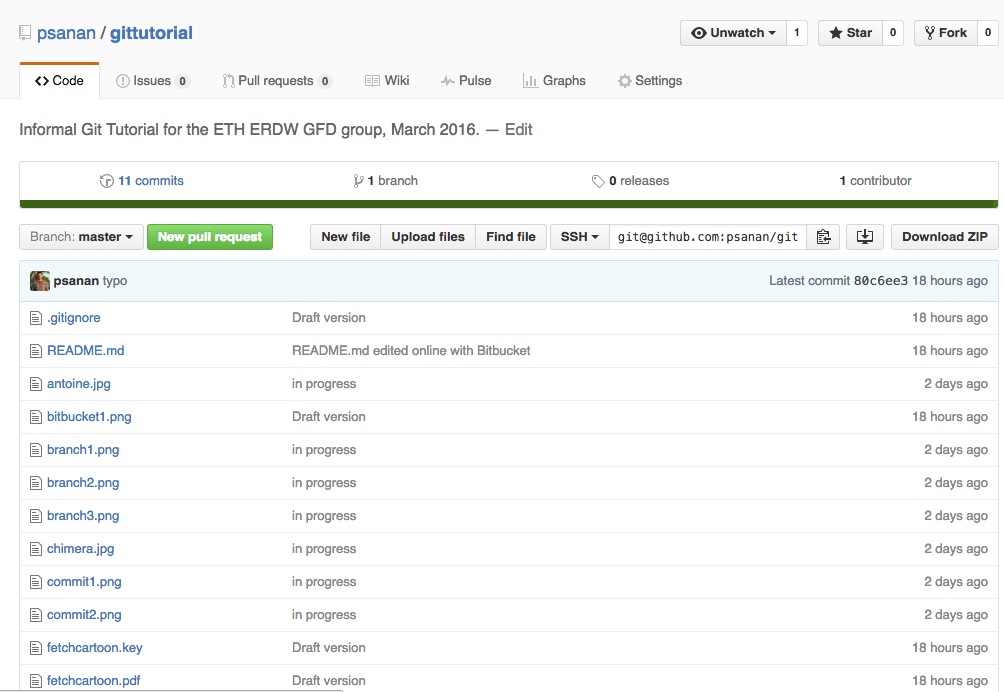
\includegraphics[scale=0.3]{github1}
\end{itemize}
\end{frame}

\begin{frame}[fragile]
\frametitle{Setting Up An Account}
\begin{itemize}
\item Bitbucket vs. GitHub? Similar in most ways, but
\begin{itemize}
\item
GitHub
\begin{itemize}
\item
is usually considered the bigger dog, with more overall users and more of a sense of community. 
\item is becoming the standard for large, open-source projects.
\end{itemize}
\item Bitbucket 
\begin{itemize}
\item will give you much more for free (unlimited private repositories) if you \textbf{sign up with an academic email address}. 
\item is my personal choice for most of my work.
\end{itemize}
\end{itemize}
\item Go to \href{https://bitbucket.org}{bitbucket.org} or \href{https://github.com}{github.com} and follow the instructions.
\item If you hate typing passwords as much as I do, it's worthwhile to set up password-free access with SSH keys\footnote{I won't cover this in detail, but ask me if you are having trouble with this} on
\href{https://confluence.atlassian.com/bitbucket/set-up-ssh-for-git-728138079.html}{Bitbucket} and
\href{https://help.github.com/articles/adding-a-new-ssh-key-to-your-github-account/}{GitHub}.
\end{itemize}
\end{frame}

\begin{frame}[fragile]
\frametitle{Putting your Project on GitHub or Bitbucket}
Follow the instructions on the site.
\begin{itemize}
\item With the website interface, create a git repository on the remote server
\item Tell your local repository about the address
\begin{lstlisting}[language=]
git remote add origin git@bitbucket.org:psanan/myproject.git
\end{lstlisting}
\item Tell some or all your local branches to track new remote branches on this remote server
\begin{lstlisting}[language=C++]
git push -u origin master
git push -u origin --all
\end{lstlisting}
\end{itemize}

Let's do this now for our demo project.

\end{frame}

\subsection{Demo: Joining a project}

\begin{frame}[fragile]
\frametitle{}
Fortunately, the workflow for joining an existing project hosted on GitHub or bitbucket is very simple!
Let's perform a typical example:
\begin{lstlisting}[language=C++]
git clone git@github.com:psanan/gittutorial-demo.git
cd gittutorial-demo
git branch psanan/helloworld
git checkout psanan/helloworld
vim hello.c
git add hello.c
vim README.md
git add README.md
git status
git commit
git push -u origin psanan/helloworld
git checkout master
vim README.md
git add README.md
git commit
git merge psanan/helloworld
git push
\end{lstlisting}
And let's take a look on GitHub
\end{frame}

\section{More selling points}
\begin{frame}[fragile]
\frametitle{Selling Points}
\begin{itemize}
\item A way to accidentally lose a lot less data
\item A handy way of dealing with code which you commonly use on multiple machines (laptop, desktop, local cluster, supercomputer)
\item A way to have a canonical version of code (on GitHub or Bitbucket)
\item Some added peace of mind that your code is backed up
\item An easy way to share your project
\item An easy way to join or use other projects
\item A nice way to organize your work
\item A good way to efficiently work with remote collaborators on code (or a paper)
\end{itemize}
\end{frame}

\section{Annoyances and Solutions}
\begin{frame}[fragile]
\frametitle{How do I remember all these stupid commands?!}
\begin{columns}
\column{0.6\textwidth}
\begin{itemize}
\item \lstinline{git help}
\item \lstinline{git status} gives you hints
\item \lstinline{git help [command]} gives you the arbitrary sub-commands and flags
\item A GUI tool can be helpful.
\begin{itemize}
\item Built-in: 
\begin{itemize}
\item
\lstinline{git gui} (construct commits) 
\item \lstinline{gitk} (see the graph)
\end{itemize}
\item Many other options:
\href{ https://git-scm.com/downloads/guis}{http://git-scm.com/downloads/guis}
\end{itemize}
\end{itemize}
\column{0.4\textwidth}

\includegraphics[width=120px]{git.png}\\
{\tiny \href{http://xkcd.com/1597/}{http://xkcd.com/1597/}}
\end{columns}
\end{frame}

\begin{frame}[fragile]
\frametitle{Merging is terrible!!}

\includegraphics[width=70px]{chimera.jpg}
\begin{itemize}
\item Yes. It's fundamentally difficult. Often it will ``just work'' with git.
\item Git cannot make many assumptions about your data.
\item Try to make contained commits so that conflicts are localized.
\item Don't let branches diverge too much. If working on a branch based on \texttt{master} for a long time, periodically merge \texttt{master} in.
\begin{lstlisting}[language=C++]
git branch psanan/my-complicated-feature
[ ... work work commit commit ..]
git checkout master
git pull
git checkout psanan/my-complicated-feature
git merge master
[ .. work work commit commit ..]
\end{lstlisting}
\item \lstinline{git status} will give you hints (like how to abort a merge).
\end{itemize}
\end{frame}

\begin{frame}[fragile]
\frametitle{Where am I?? What's going on??}
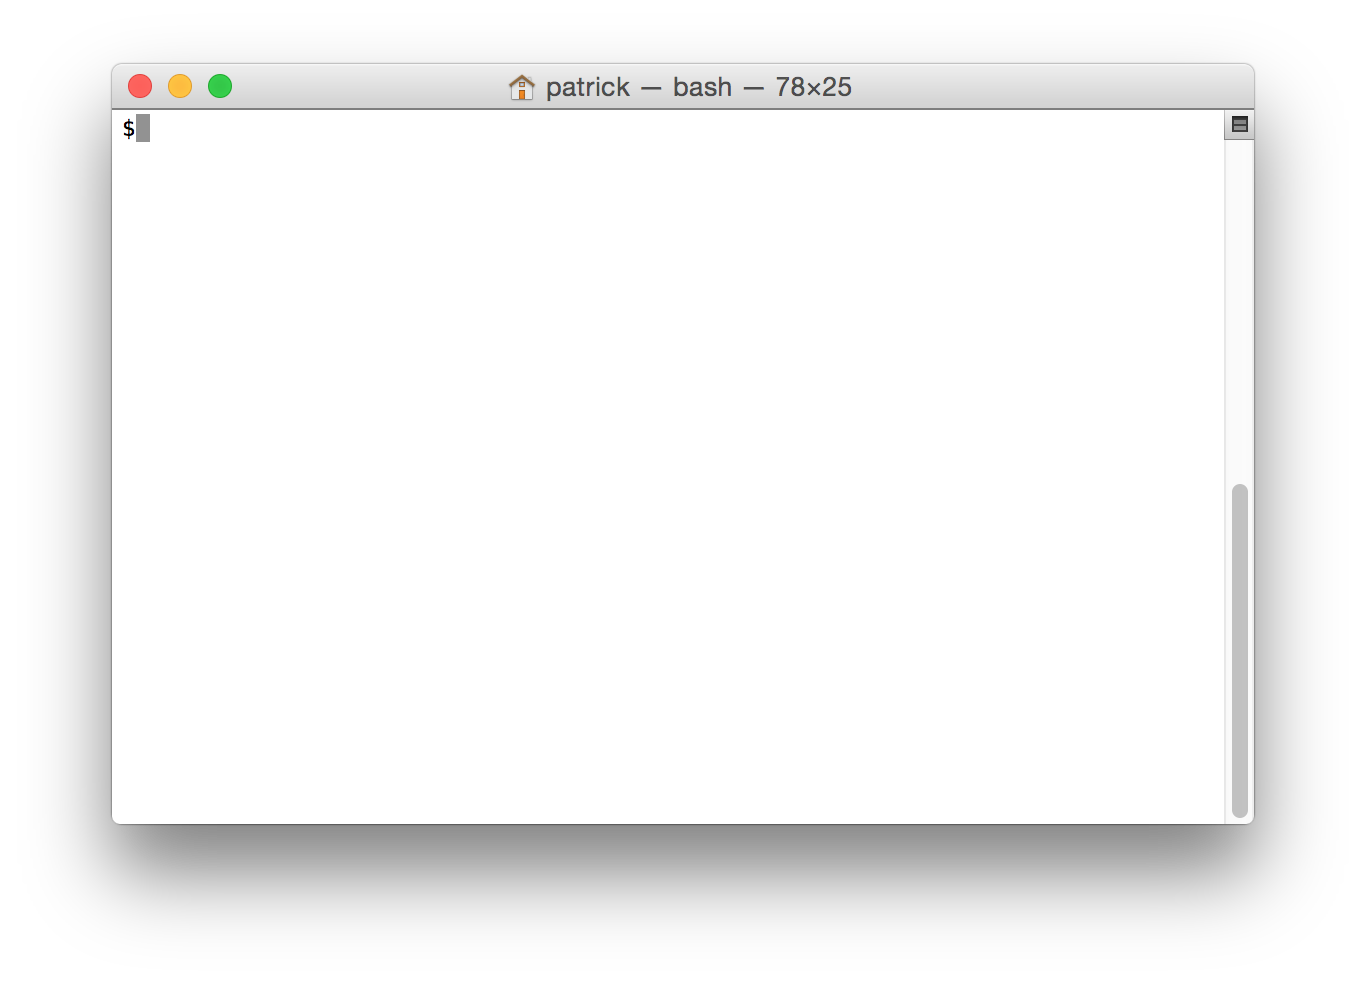
\includegraphics[width=100px]{term}\scalebox{3}{???}
\begin{itemize}
\item Turn on colors (see setup earlier)
\item 
Remember useful git commands:
\begin{itemize}
\item \lstinline{git status}
\item \lstinline{git diff [filename]}
\item \lstinline{git fetch}
\item \lstinline{git log -10}
\item \lstinline{git branch -avv} (See \lstinline{git help branch} for the options)
\item \lstinline{git remote -vv}
\end{itemize}
\item Use a \href{https://raw.githubusercontent.com/git/git/master/contrib/completion/git-prompt.sh}{terminal prompt which shows git status}\footnote{follow link or google ``git prompt'' which should bring up a commonly-used script called \texttt{git-prompt.sh}}.
\item Visualize your project with a GUI tool or with Bitbucket/GitHub
\end{itemize}
\end{frame}

\begin{frame}[fragile]
\frametitle{Uncommitted changes, need to work on another branch}
\begin{itemize}
\item Option 0: finish your current commit
\item Option 1: clone a new copy of the code
\begin{lstlisting}[language=C++]
cd .. 
git clone git@github.com:psanan/myproject.git myproject-copy
cd myproject-copy
git checkout some-other-branch
\end{lstlisting}
\item Option 2: Stash the changes with \lstinline{git stash}
\begin{lstlisting}[language=C++]
git stash
git checkout some-other-branch
...
git checkout my-working-branch
git stash apply
\end{lstlisting}
\textbf{dangerous} because you need to remember where you were.
\item Option 3: Throw away all your changes with \lstinline{git reset --hard HEAD} (\textbf{dangerous: this deletes data!})
\end{itemize}
\end{frame}

\begin{frame}[fragile]
\frametitle{The End}

For More Help:
\begin{itemize}
\item This presentation: \href{https://bitbucket.org/psanan/gittutorial}{https://bitbucket.org/psanan/gittutorial}
\item
The Git Book: \href{https://git-scm.com/book}{git-scm.com/book}
\item 
Tutorials on GitHub and Bitbucket
\item 
Beware \href{https://www.stackoverflow.com}{StackOverflow}: do not panic and start pasting mysterious commands, and note that a lot of the advice is specific to old versions of git.
\item \href{mailto:patrick.sanan@erdw.ethz.ch}{patrick.sanan@erdw.ethz.ch} (or gchat, or skype, or come to my office [H23])
\end{itemize}
\vspace{50px}
{\tiny ``... git actually has a simple design, with stable and reasonably well-documented data structures. 
In fact, I'm a huge proponent of designing your code around the data, rather than the other 
way around, and I think it's one of the reasons git has been fairly successful ... I will, in 
fact, claim that the difference between a bad programmer and a good one is whether [he or she] 
considers [his or her] code or [his or her] data structures more important. Bad programmers worry 
about the code. Good programmers worry about data structures and their relationships.''\\
--\href{http://lwn.net/Articles/193245/}{Linus Torvalds, 2006}
}
\end{frame}
\end{document}
